\section{Induce subdivision}
\label{section:pl-subdivide}

The goal of subdividing $N$ is to create and identify handle attachment sites analogous to the face, edge, and vertex blocks of Chapter \ref{chapter:smooth}.
We use a similar technique to that found in Chapter \ref{chapter:smooth}, iteratively subdividing the tetrahedra of $N$ by certain preimages of $f$.
Tetrahedron subdivisions are compatible, i.e.\ tetrahedron subdivisions fit together exactly as the undivided tetrahedra do inside of $N$.

Let $\sigma$ be a tetrahedron of $N$ and let $s$ be a line segment in the plane such that $s\cap f(\sigma)$ is nonempty, the endpoints of $s$ are outside of $f(\sigma)$,  and $s\cap f(\sigma)$ is a line segment in $f(\sigma)$ disjoint from any vertices or crossings of $f(\sigma)$.
Figure \ref{fig:standard-position-intersection} demonstrates the possible configurations of these line segments, and shows that their preimages inside of $\sigma$ are triangles and quads.
We refer to these preimages as \emph{exterior triangles} and \emph{exterior quads}.
When a pair of these preimages intersect, the intersection is a line segment with endpoints interior to a pair of triangles of $\sigma^2$.

\begin{figure}[h!]
	\centering
	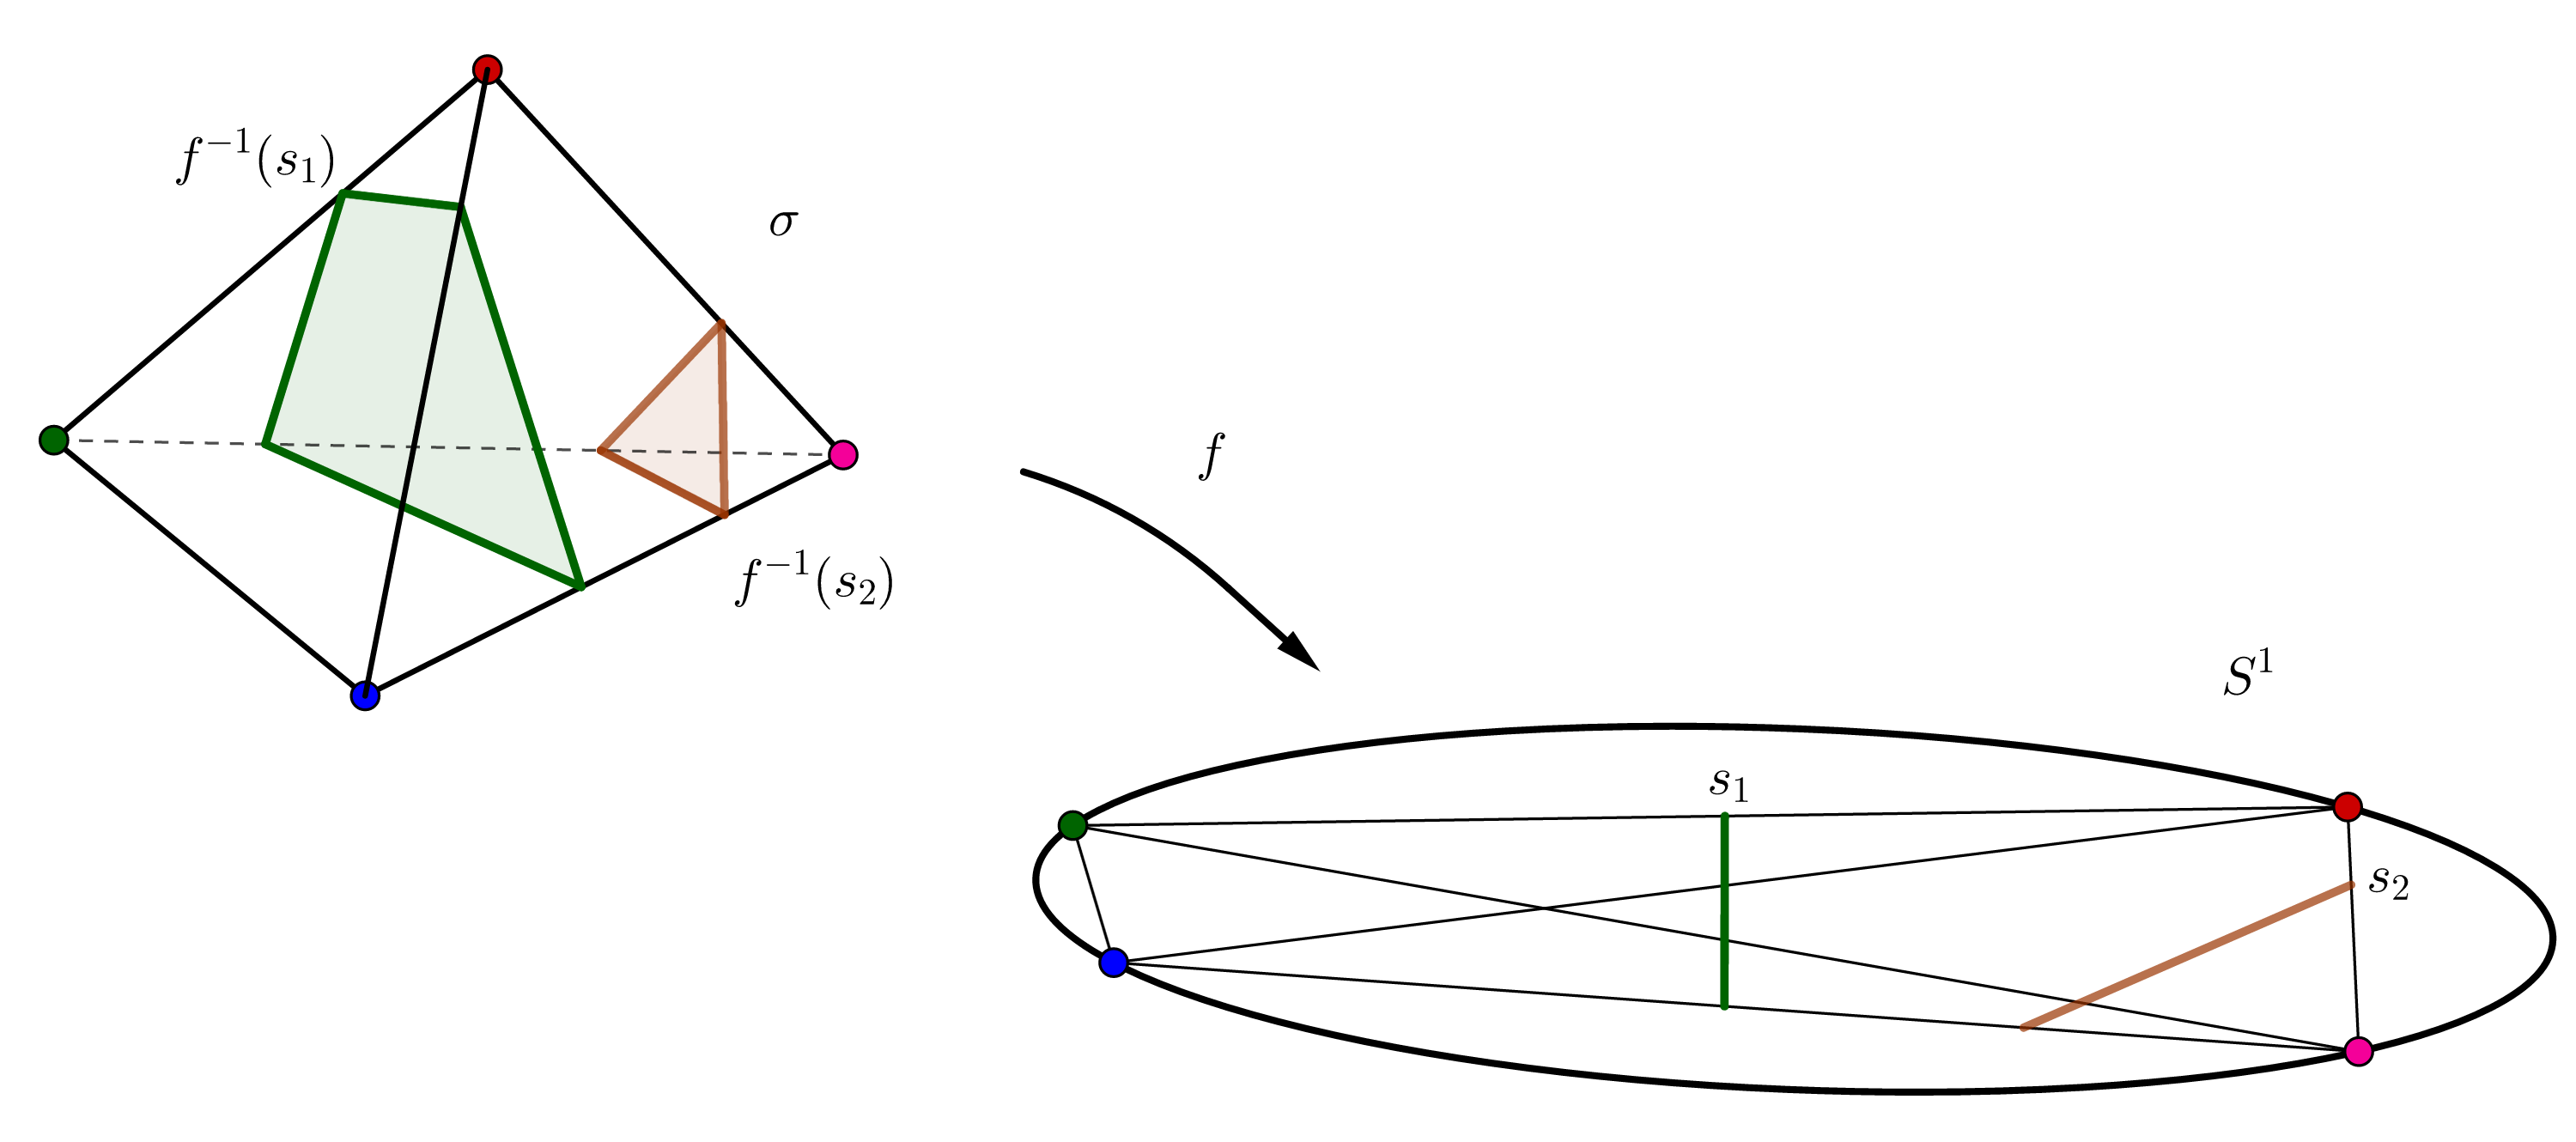
\includegraphics[width=0.9\textwidth]{figures/standard-position-intersection.png}
	\caption{
		\textbf{A tetrahedron $\sigma$ in standard position, intersecting edges, and preimage triangles and quads.}
		An intersecting edge separates the vertices of $\sigma$.
		If one is separated from the other three, its preimage is a triangle.
		If the vertices are separated into two pairs of two, the preimage is a quad.
	}
	\label{fig:standard-position-intersection}
\end{figure}

For each $\sigma\in N^3$ and each edge $e$ of $N^1$ such that $e\notin\sigma^1$, $f(e)$ is a line segment in the plane that is either disjoint from $f(\sigma)$ or induces an exterior triangle or quad in $\sigma$.
There are two edges of $\sigma$ whose preimages in $\sigma$ form \emph{interior triangles}.
These are the preimages of the edges of $\sigma$ that map through $f$ across $f(\sigma)$ as in Figure \ref{fig:standard-position}, and we refer to these edges as \emph{interior edges}.
The three edges of the interior triangle induced by $e$ are $e$ itself along with a pair of edges that bisect the triangles of $\sigma$ not containing $e$ as an edge.
The three vertices of the interior triangle induced by $e$ are the two vertices of $\sigma$ that are the endpoints of $e$ along with a third vertex located in the edge of $\sigma$ opposite $e$.
Figure \ref{fig:standard-position-interior-exterior} shows one interior triangle along with its possible intersections with exterior triangles and quads.
The interior triangles of $\sigma$ always intersect in a line segment with endpoints inside of the interior edges of $\sigma$, shown in Figure \ref{fig:standard-position-interior-interior}

\begin{figure}[h!]
	\centering
	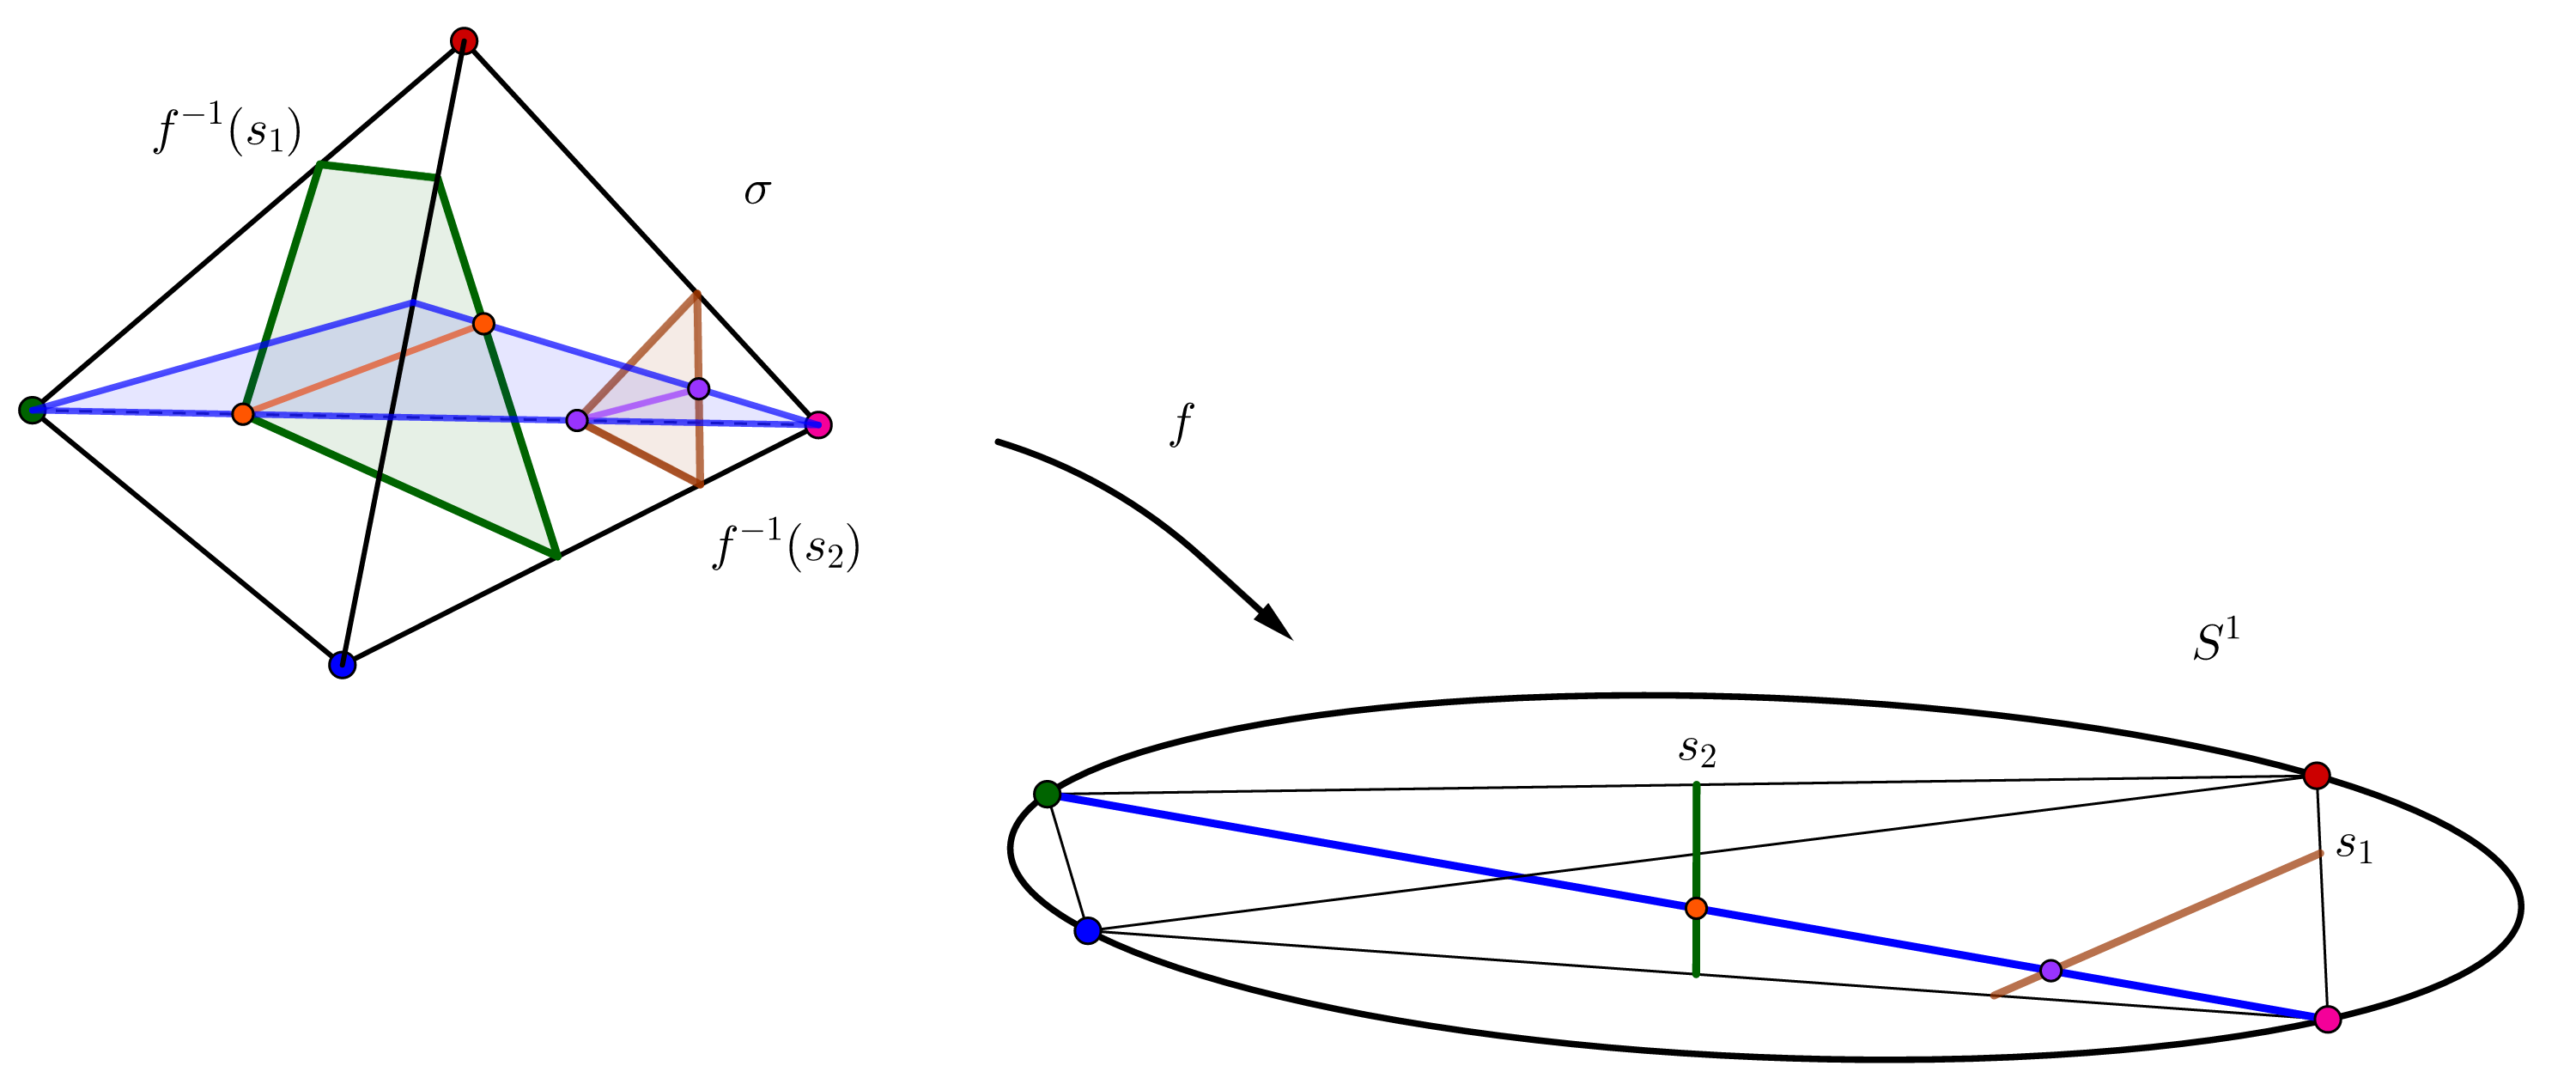
\includegraphics[width=0.9\textwidth]{figures/standard-position-interior-exterior.png}
	\caption{
		\textbf{A tetrahedron $\sigma$ in standard position, one interior triangle, one exterior triangle, and one exterior quad.}
		There are two special preimage triangles in $\sigma$, called \emph{interior triangles}, that occur as the preimages of the edges of $\sigma$ that map through $f$ across $f(\sigma)$ as in Figure \ref{fig:standard-position}.
	}
	\label{fig:standard-position-interior-exterior}
\end{figure}

\begin{figure}[h!]
	\centering
	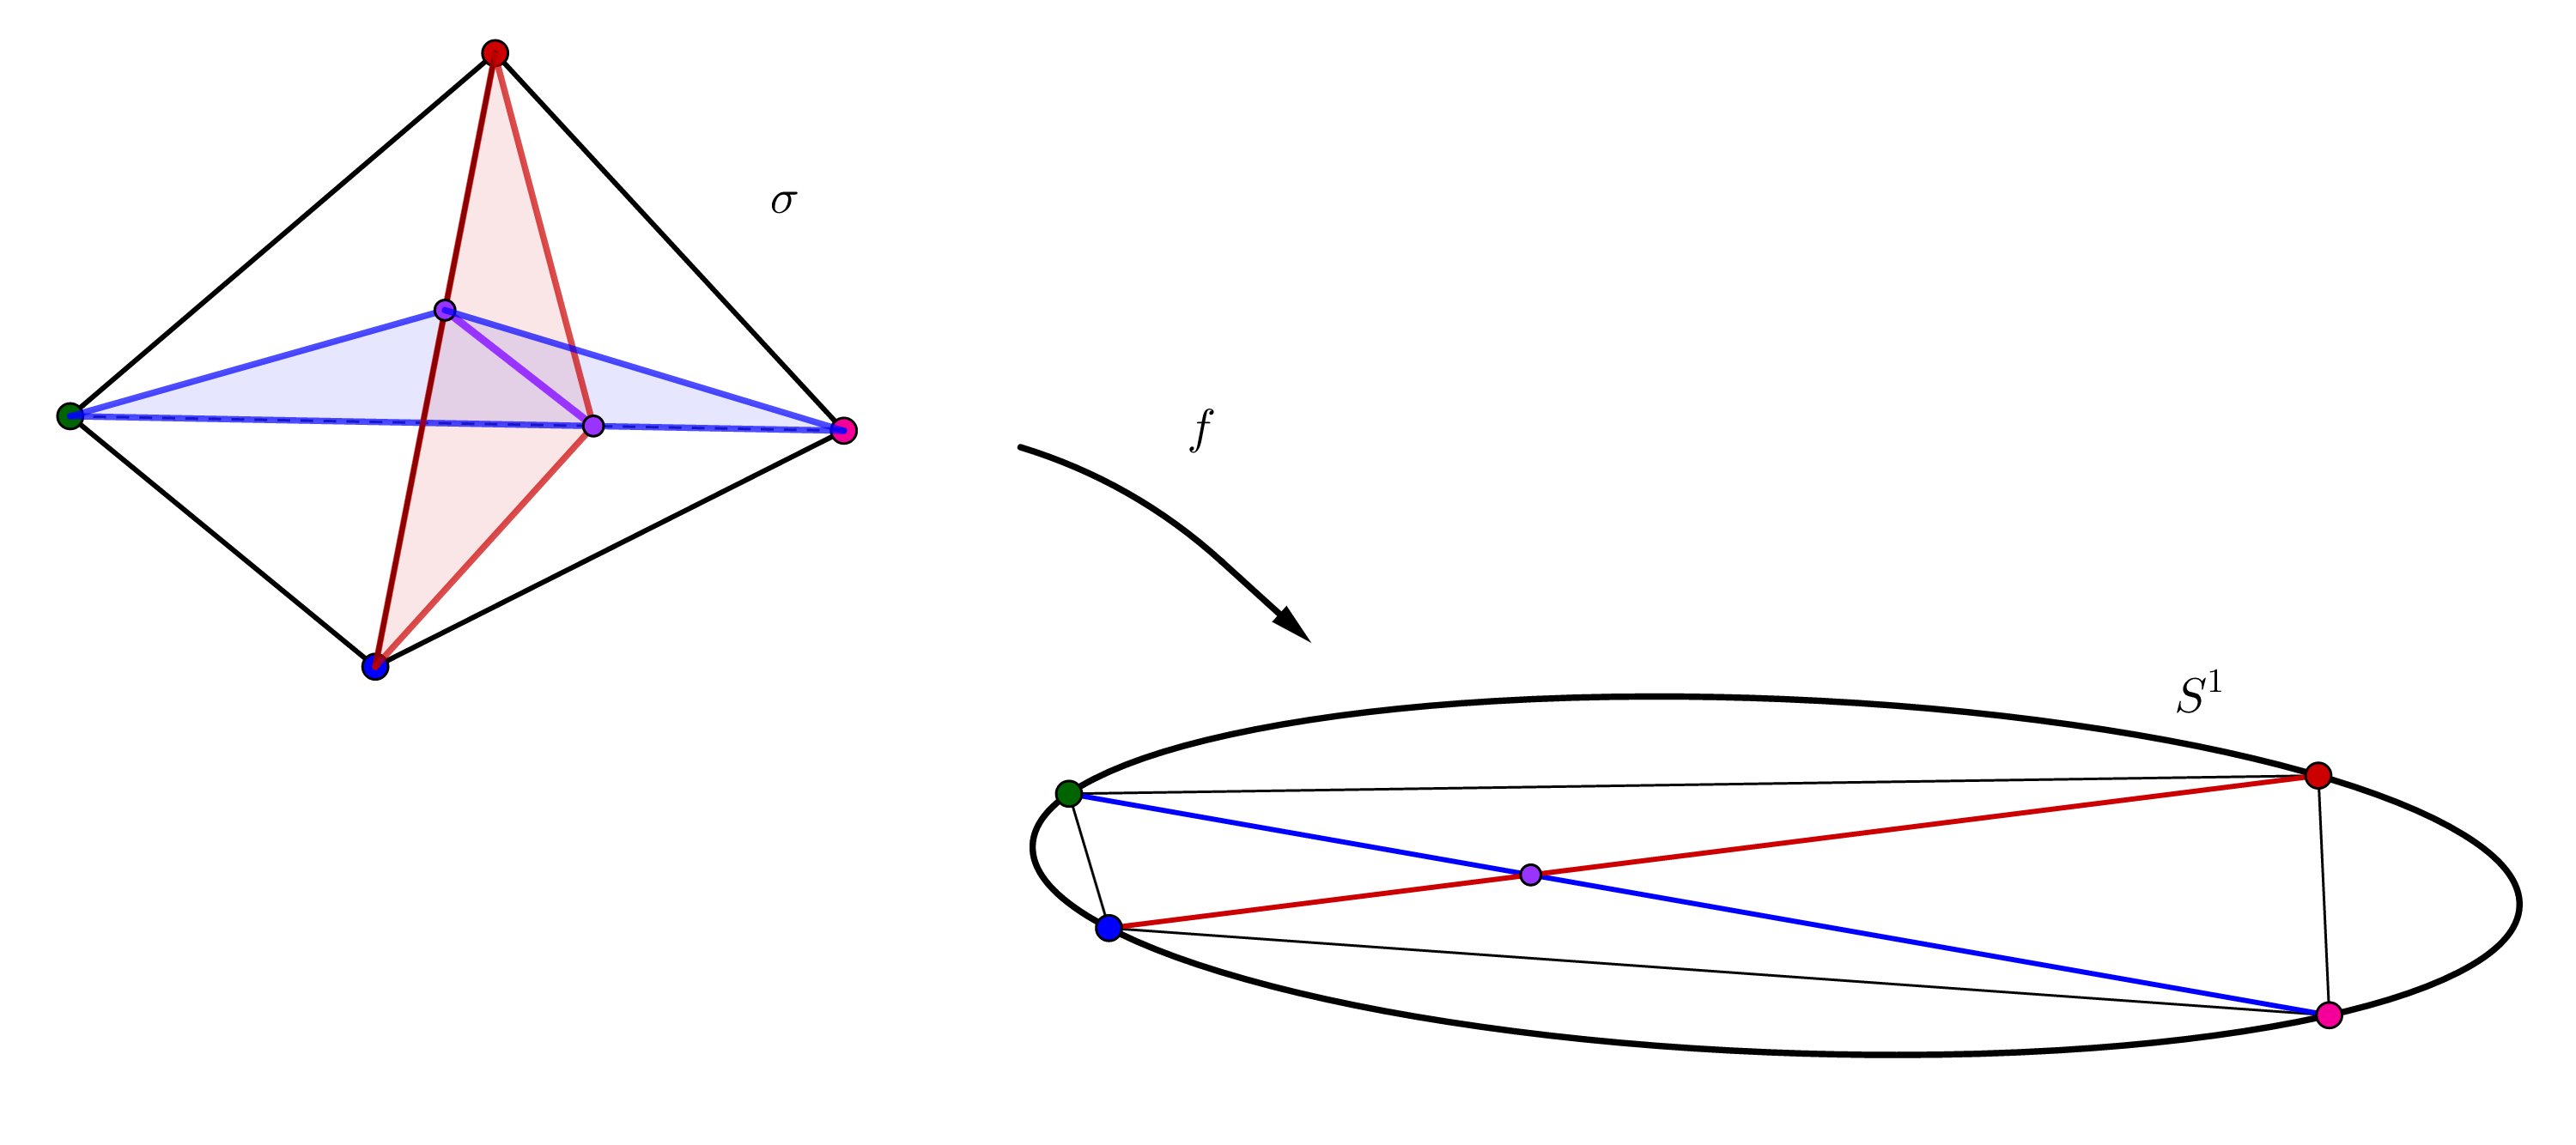
\includegraphics[width=0.9\textwidth]{figures/standard-position-interior-interior.png}
	\caption{
		\textbf{A tetrahedron $\sigma$ in standard position with both interior triangles.}
		As in Figure \ref{fig:standard-position-interior-exterior}, but displaying both interior triangles.
	}
	\label{fig:standard-position-interior-interior}
\end{figure}

Recall that the goal of this subdivision is to identify combinatorial analogues for the face, edge, and vertex blocks of Chapter \ref{chapter:smooth}.
If we were to subdivide $N$ using the quads and triangles induced by the edges of $N$, such blocks are ill-defined.
We amend this by introducing a set of line segments analogous to the sleeves of Section \ref{section:smooth-decompose}.

For each edge $e$ of $N^1$, consider $e_\varepsilon^+ = s(e+\varepsilon_e e_\perp)$ and $e_\varepsilon^- =s(e-\varepsilon_e e_\perp)$, secants in the circle that are parallel to $f(e)$ and located a small orthogonal distance away from $f(e)$.
Here we are using $s(\cdot)$ as a function that extends and trims line segments in the plane into secants in the circle.
We require that, for each $e\in N^1$, $\varepsilon_e$ is small enough that the rectangle $R_e$ in the plane defined by $e_\varepsilon^+$ and $e_\varepsilon^-$ does not fully contain $g_\varepsilon^\pm$ for any $g\in N^1$.
This requirement also ensures that the only crossings of $f(N^1)$ contained in $R_e$ are crossings involving $e$.
The segments $e_\varepsilon^\pm$ for each $e\in N^1$ are called \emph{sleeve segments}, and their preimages form exterior triangles and quads inside of the tetrahedra of $N$, as shown in Figure \ref{fig:pl-sleeves}.

\begin{figure}[h!]
	\centering
	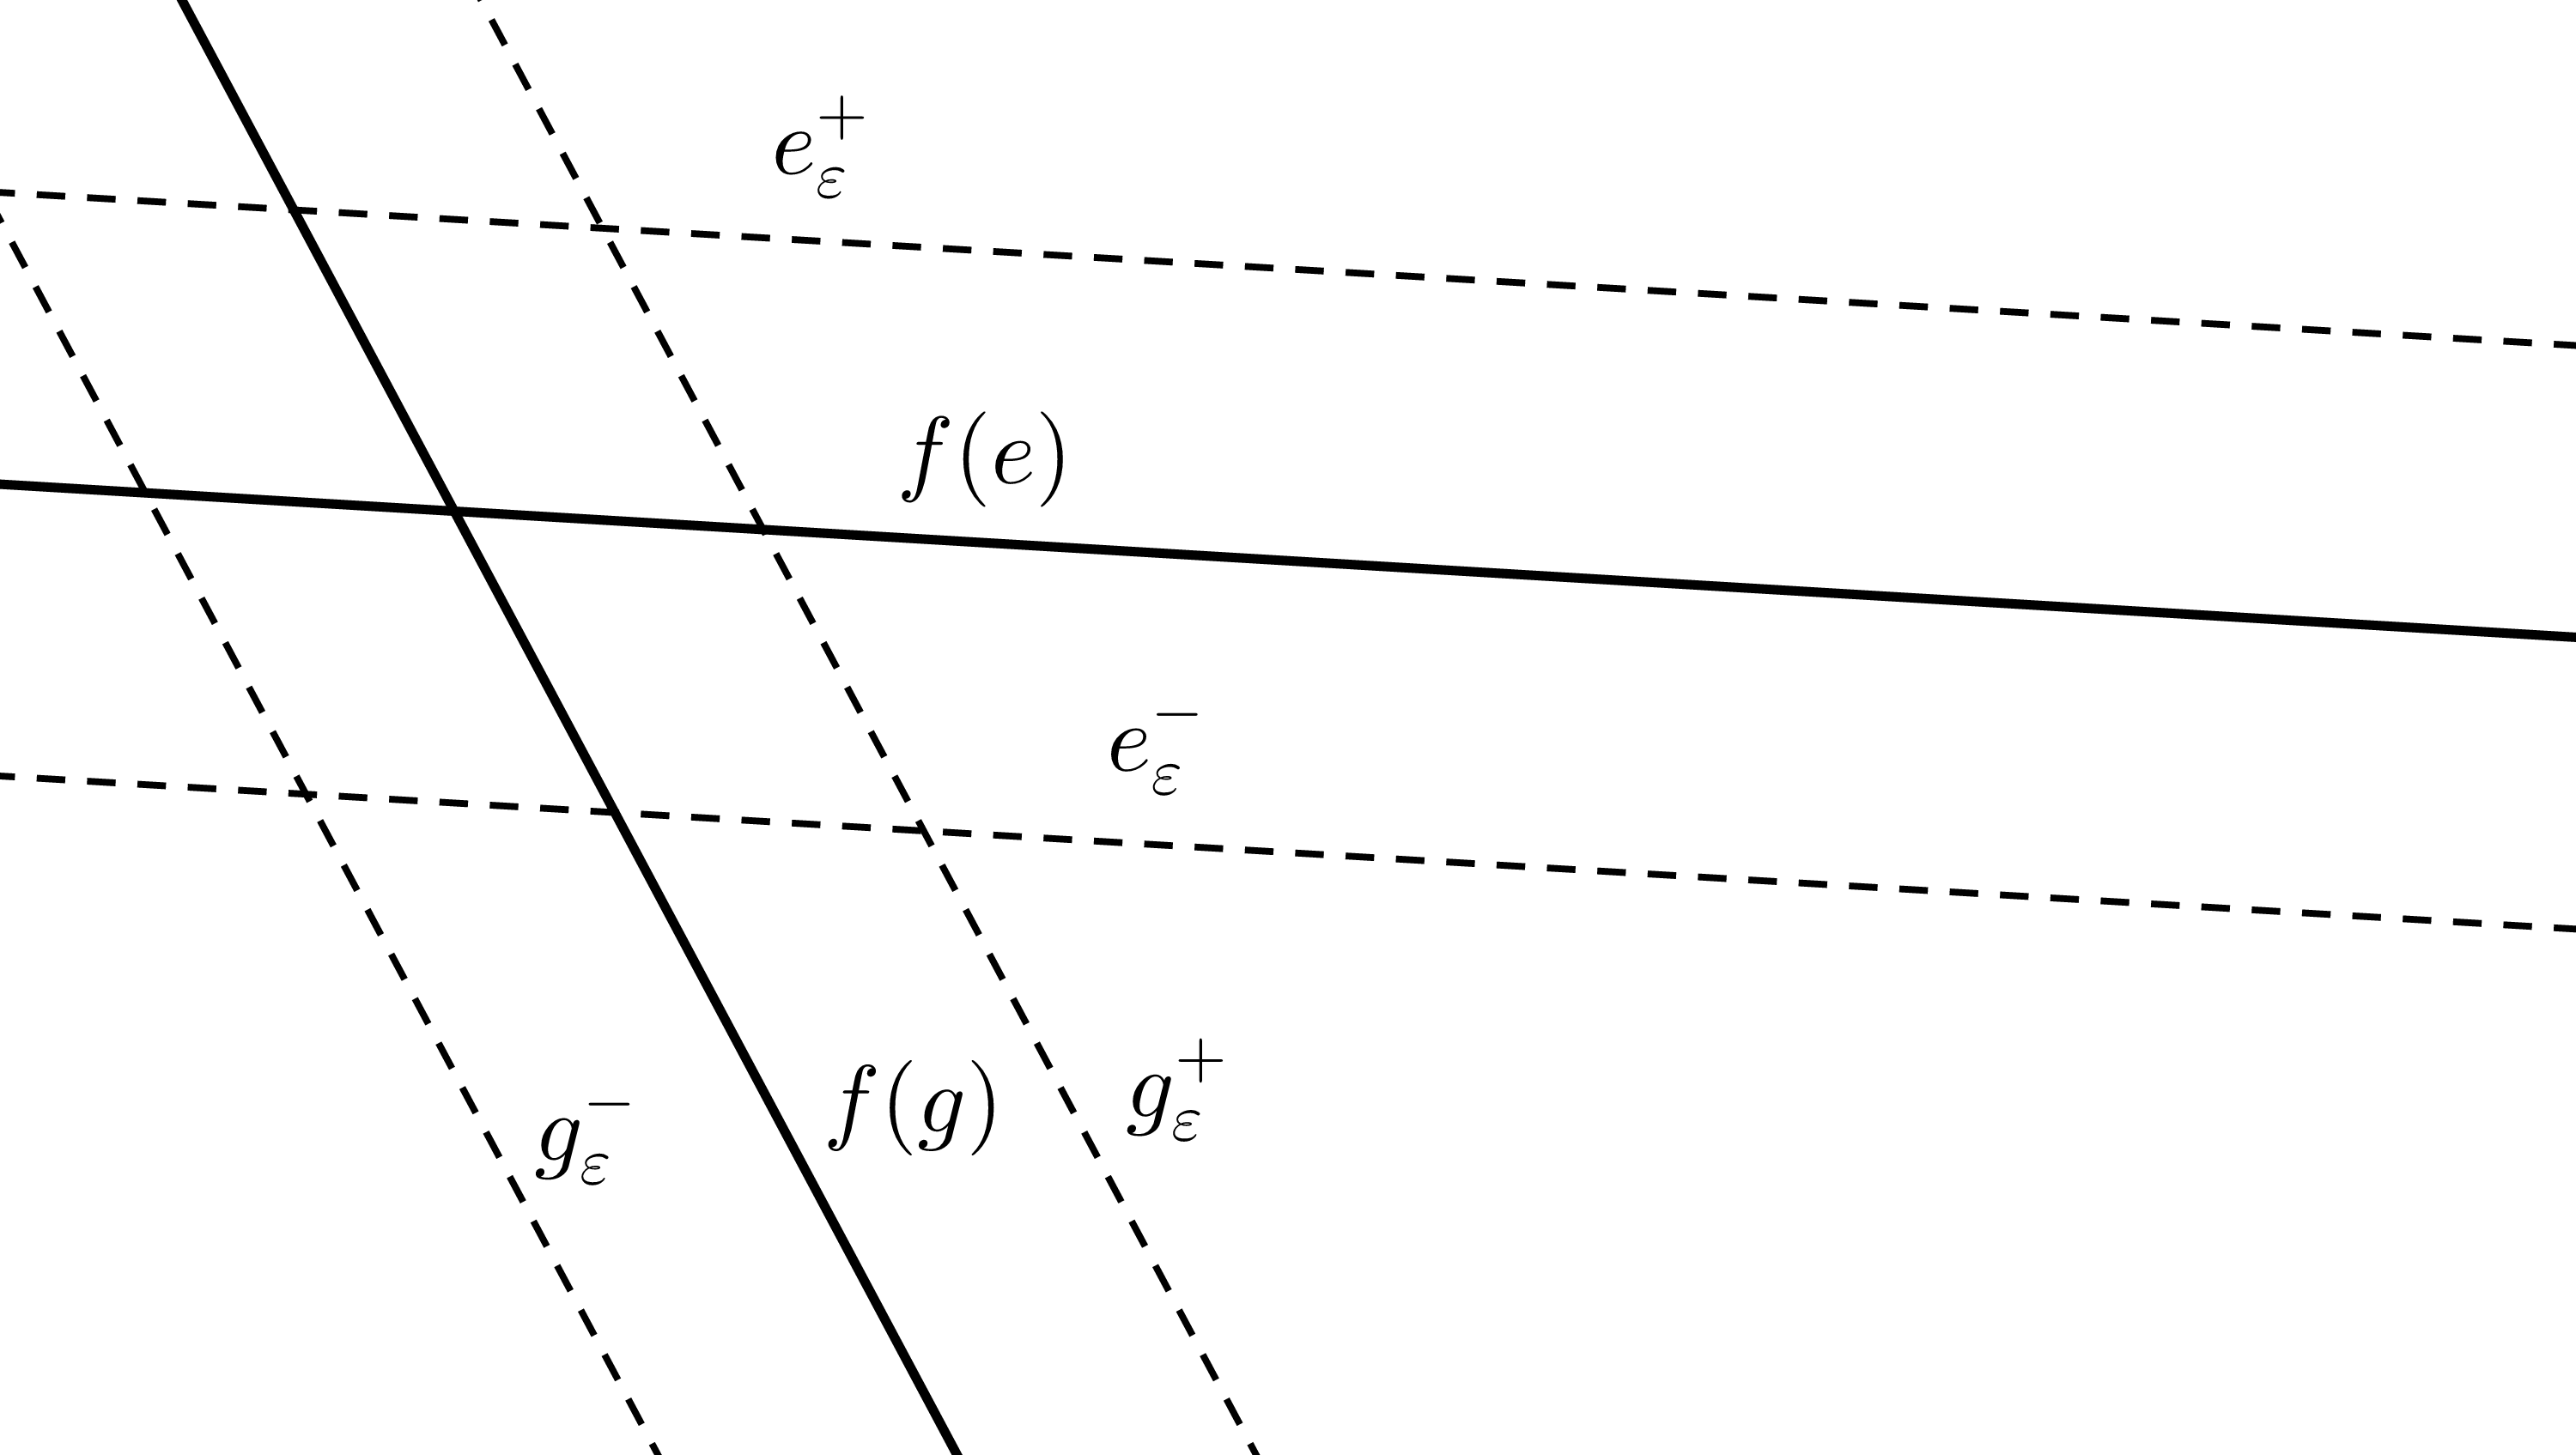
\includegraphics[width=0.9\textwidth]{figures/pl-sleeves.png}
	\caption{
		\textbf{A pair of sleeve segments in the plane.}
		We show a pair of edges projections $f(e)$ and $f(g)$ in the plane, along with their associated sleeve segments.
		Sleeve segments are necessary to ensure well-defined face, edge, and vertex block analogues in the subdivision of $N$.
	}
	\label{fig:pl-sleeves}
\end{figure}

Take $S$ to be the set of line segments in the plane that consists of $f(e)$ for each $e\in N^1$ along with the sleeve segments $e_\varepsilon^\pm$.
For each tetrahedron $\sigma$ of $N$, the triangles, quads, and intersections of $f\inv S\cap\sigma$ define a subdivision of $\sigma$ into a cell complex.
Iteration of this subdivision in Algorithm \ref{alg:subdividing-manifold} across all tetrahedra of $N$ yields a 3--dimensional cell complex $M$.

We subdivided $N$ into $M$ in order to identify analogues to the face, edge, and vertex blocks of Chapter \ref{chapter:smooth}.
The analogous blocks are defined exactly as they were in Chapter \ref{chapter:smooth} --- the sleeve segments subdivide the plane into regions homeomorphic to disks, those disks are classified by whether they contain a crossing of $f(N^1)$, intersect $f(N^1)$ but do not contain a crossing, or do not intersect $f(N^1)$ at all.
The preimage of a region that contains a crossing is a \emph{combinatorial vertex block}, the preimage of a region that intersects $f(N^1)$ but does not contain a crossing is an \emph{combinatorial edge block}, and the preimage of a region that is disjoint from $f(N^1)$ is a \emph{combinatorial face block}.
Symmetric names are used for the regions that these blocks project onto --- combinatorial face (resp. edge, vertex) blocks map through $f$ to \emph{combinatorial face (}resp. \emph{edge, vertex) regions}.
Figure \ref{fig:pl-regions} illustrates the regions in the plane that produce such blocks.
These preimages exhaust the cells of $M$, providing a decomposition into subcomplexes.
This decomposition is not a partition --- some cells are assigned to more than one block.
Such an assignment happens precisely when a cell is mapped through $f$ to the shared boundary of different combinatorial regions.

%Note: we 'need' to include S^1\in\RR to actually form the regions discussed, but that's pretty obvious so we won't address it unless requested.

\begin{figure}[h!]
	\centering
	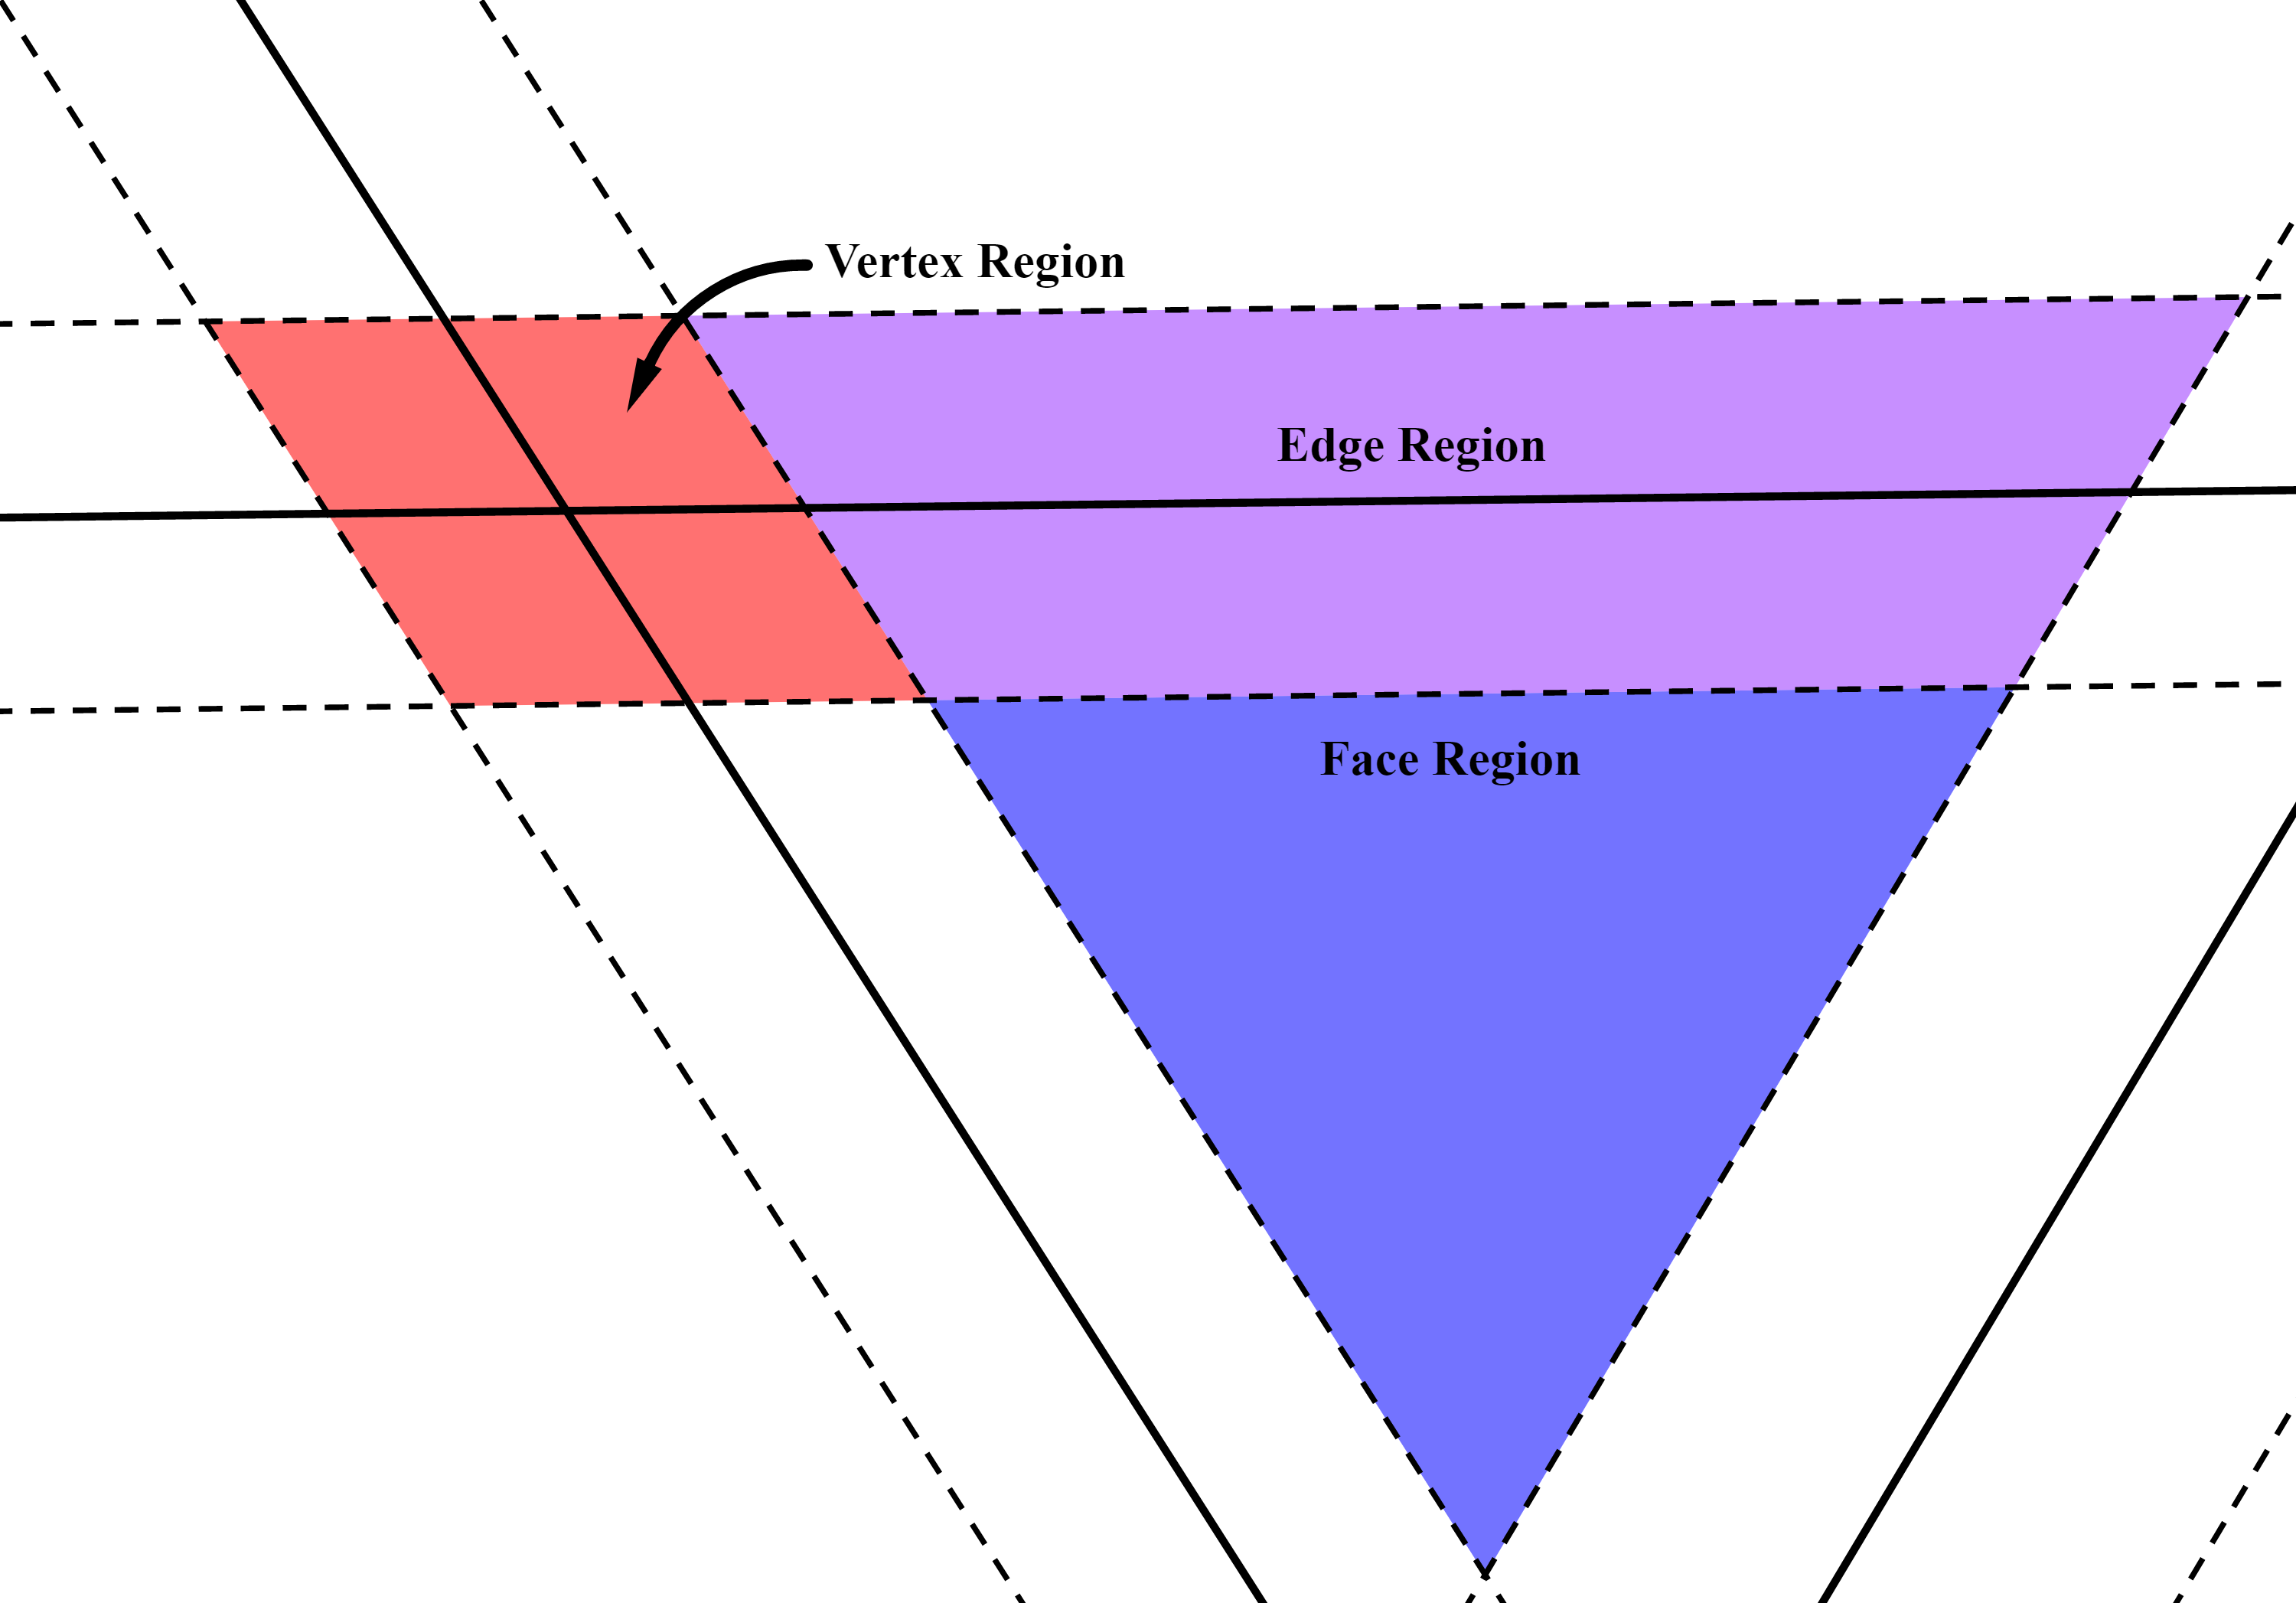
\includegraphics[width=0.9\textwidth]{figures/pl-regions.png}
	\caption{
		\textbf{Regions in the plane that correspond to combinatorial vertex, edge, and face block.}
		The sleeve segments provide the same functionality as the sleeves in Chapter \ref{chapter:smooth}, in that the preimages of the regions they form behave similarly to the vertex, edge, and face blocks defined in Chapter \ref{chapter:smooth}.
	}
	\label{fig:pl-regions}
\end{figure}

The Cartesian product of a pair of cell complexes is again a cell complex, so we form the base 4--dimensional cell-complex to which we attach handles as $M\times\Ilit$.
Every cell of $M\times\Ilit$ is homeomorphic to a disk, so we form a 4--manifold triangulation $W$ as a subdivision of $M\times\Ilit$.
This triangulation is obtained by inductively subdividing each cell of $M\times\Ilit$ that is not a simplex.

\begin{algorithm}[h!]
	\caption{Subdividing $N$}
	\label{alg:subdividing-manifold}
	\KwData{A closed, orientable 3--manifold triangulation $N$ with subdividing map $f:N\to\RR$}
	\KwResult{A closed, orientable 3--dimensional cell complex $M$}
	\Begin{
		$S = \{f(e)\;|\;e\in N^1\}\cup\{e_\varepsilon^\pm\;|\;e\in N^1\}$\;
		\ForEach{tetrahedron $\sigma$ of $N^3$}{
			\ForEach{segment $s$ of $S$}{
				$\delta = $ the intersection of $\sigma$ with $f\inv s$\;
				replace $\sigma$ with the 3--dimensional cell complex obtained as $\sigma$ subdivided by $\delta$\;
			}
		}
	}
\end{algorithm}

%Each 3--cell of $M$ maps through $f$ to a connected component of $f(N)\setminus f(N^1)$.
%Let $r$ be a connected component of $f(N)\setminus f(N^1)$.
%Then $f\inv(r)$ is a collection of 2-- and 3--cells in $M$ that form a  
%Their is a correspondence between the 3--cells of $M$ and the connected components of $f(N)\setminus f(N^1)$, and that correspondence 
%
%Decomposition of $\RR$ is done through $f(N_1)$.
%A point in $f(N_1)$ is the image of either a vertex, exactly one edge, or exactly two edges (i.e.\ is an edge crossing), so we refer to these as the \emph{vertices}, \emph{edges}, and \emph{crossings} of the decomposition.
%Because $f(N)\setminus f(N_1)$  is a disjoint collection of simply connected regions, we call the connected components of $f(N)\setminus f(N_1)$ the \emph{faces} of the decomposition.
%
%We construct our subdivision of $N$ using the decomposition component preimages.
%The preimage of a face component defines substructures analogous to face blocks, of edge components to edge blocks, and vertices and crossings to vertex blocks.
%Inside of an individual tetrahedron of $N$, edge and crossing preimages are well-defined, supplying a natural subdivision of $N$ into a cell complex.
%Then, the subdivision of a cell complex into a triangulation is well-defined.
%
%The algorithm presented in this section takes as input a closed, orientable 3--manifold triangulation $N$ and a projection $f:N\to\RR$ and produces as output a closed, orientable 3--dimensional cell complex $M$ that is a subdivision of $N$.
%Furthermore, the 3--cells of $M$ are partitioned into subsets that serve the same purpose as the face blocks of Chapter \ref{chapter:smooth}: attaching regions for 2--handles.
%This 3--cell partitioning also induces a partition on the 2--cells of $M$ into subsets that are either interior to face blocks, or subsets that serve the same purpose as the edge blocks of Chapter ~\ref{chapter:smooth}, i.e.\ buffers between face blocks.
%
%
%
%
%
